%% This is file `DEMO-TUDaThesis.tex' version 4.03 (2025-04-02),
%% it is part of
%% TUDa-CI -- Corporate Design for TU Darmstadt
%% ----------------------------------------------------------------------------
%%
%% Copyright (C) 2018--2025 by Marei Peischl <marei@peitex.de>
%%
%% ============================================================================
%% This work may be distributed and/or modified under the
%% conditions of the LaTeX Project Public License, either version 1.3c
%% of this license or (at your option) any later version.
%% The latest version of this license is in
%% http://www.latex-project.org/lppl.txt
%% and version 1.3c or later is part of all distributions of LaTeX
%% version 2008/05/04 or later.
%%
%% This work has the LPPL maintenance status `maintained'.
%%
%% The current maintainer of this work is
%%   Marei Peischl <tuda-ci@peitex.de>
%%
%% The development repository can be found at
%% https://github.com/tudace/tuda_latex_templates
%% Please use the issue tracker for feedback!
%%
%% If you need a compiled version of this document, have a look at
%% http://mirror.ctan.org/macros/latex/contrib/tuda-ci/doc
%% or at the documentation directory of this package (if installed)
%% <path to your LaTeX distribution>/doc/latex/tuda-ci
%% ============================================================================
%%
% !TeX program = lualatex
%%

% Enable PDF/A via pdfmanagement and no longer via pdfx
\DocumentMetadata{
	pdfstandard=a-2b,
	pdfversion=1.7,% 2.0 is possible as well, but PDF/A-2b requires < 2.0
	lang=en,
}

\documentclass[
	german,% Main language as global option
	accentcolor=9c,% Choose accent color: For a list of available colors see the full tudapub documentation
	ruledheaders=section,% Section levels above this one will follow the ruled layout
	class=report,% Choose the base document class. Will choose the matching KOMA-Script class
	thesis={type=bachelor},% Thesis. For PhD thesis have a look at DEMO-TUDaPhd example file
	fontsize=11pt,% Basic font size. CI default setting of 9pt is too small for theses
	parskip=half-,% Use a parskip instead of indent, see KOMA-Script documentation
	custommargins=false,% Calculate margins using typearea
	marginpar=false,% Disable marginpar
	BCOR=0mm,% Binding correction
% 	accept-missing-logos=true,% No error in case logo files are not available
 	logofile=tools/logo-installation/TUDa-logos/tuda_logo.png,% In case logo should be replaced
]{tudapub}


%%%%%%%%%%%%%%%%%%%
% Language setup
%%%%%%%%%%%%%%%%%%%
\usepackage[english]{babel}
\usepackage{microtype}
\usepackage[autostyle]{csquotes}% \enquote, to simplify use of quotation marks
\usepackage{caption} 
\usepackage{wrapfig}
\usepackage{ amssymb }


%%%%%%%%%%%%%%%%%%%
% Bibliography
%%%%%%%%%%%%%%%%%%%
\usepackage[sorting=none, citestyle=numeric-comp]{biblatex}
\addbibresource{ref.bib}% File name of BibTeX database

%%%%%%%%%%%%%%%%%%%
% Package suggestions for tables
%%%%%%%%%%%%%%%%%%%
\usepackage{array}% Fundamental tools for tables. Is automatically loaded by the following packages
%\usepackage{tabularx}% Tables with flexible columns to achieve fixed width
%\usepackage{longtable}% Tables across multiple pages
%\usepackage{xltabular}% Tables with fixed width spanning multiple pages
%\usepackage{booktabs}% Improved layout for horizontal rules in tables

%%%%%%%%%%%%%%%%%%%
% Package suggestions math
%%%%%%%%%%%%%%%%%%%
\usepackage{mathtools}% Extended version of amsmath
\usepackage{amssymb}% Additional symbols
\usepackage{siunitx}% Numbers and Units

\usepackage{subcaption}
\usepackage{tikz}
\usepackage{pgfplots}
\pgfplotsset{compat=1.18} % You can adjust the version as needed


\hypersetup{% Metadata adjustments, in case these are not set, the data provided for \maketitle will be used
	pdfauthor=Marei Peischl (peiTeX),
	pdfcreationdate=2024-05-03,
	pdfkeywords={TU Darmstadt; Corporate Design; LaTeX}
}

\title{Removal of undesired resonances of Terahertz antennas by inclusion of resistive feeds}
\author{Jakob Schmidt}
\reviewer{Prof. Dr. rer. nat. Sascha Preu \and Florian Bek M.Sc.}

% The following elements will be placed on the title page
\department{etit}% If defined the shorthand will be replaced by the full name otherwhise it's used directly.
\institute{Institute for Microwave Engineering and Photonics}
\group{Terahertz Devices and Systems}

\submissiondate{\today}
\examdate{\today}

%\tuprints{printid=XXXX,year=2022,license=cc-by-4.0}% License information for TUprints

\begin{document}

\maketitle

%% The affidavit was deactivated by default at the request of Department II.
%% According to the department, the legally binding text can be found at https://www.tu-darmstadt.de/studieren/studierende_tu/studienorganisation_und_tucan/hilfe_und_faq/artikel_details_de_en_37824.de.jsp
%%  The docx file should be used, printed out, signed, scanned and then integrated.
%% The easiest way to do this is to use the pdfpages package.
%%
%% For compatibility reasons for the other templates, the function is still available.
%% \affidavit[signature-image={\includegraphics[width=\width,height=1cm]{example-image}}, <there may be additional options here>]

\tableofcontents
% Additional lists like \listoffigures or acronyms might be added here
\listoffigures
\newpage

\chapter{Introduction}
In between the microwave and infrared (IR) frequencies of the electromagnetic (EM) spectrum lies Terahertz (THz) radiation (see Figure \ref{thz_overview}) \cite{zhangIntroductionTHzWave2010}. THz radiation refers to the frequency (wavelength) spectrum ranging from \num{100} \si{\giga\hertz} (\num{3} \si{\milli\meter}) up to \num{10} \si{\tera\hertz} (\num{30} \si{\micro\meter}). 
This part of the spectrum is often referred to as the \enquote{THz gap} (e.g. see \cite{dhillon2017TerahertzScience2017, williamsFillingTHzGap2006, zhangAdvancesTerahertzTechnology2021}), since efficient sources and detectors are still limited compared to adjacent frequency ranges \cite{perkowitzNavigatingTerahertzGap2020}. Over the last decades, significant progress has been made in bridging this gap from both the electronic and photonic side. Advances have been made by extending the high frequency cut-off in purely electronic RF devices, decreasing the lower cut-off frequencies of purely optical IR devices or even by combining the two approaches \cite{preuTunableContinuouswaveTerahertz2011}. A particularly versatile and widely used technique enabled by these developments is THz time-domain spectroscopy (THz-TDS). In THz-TDS, ultrafast femtosecond lasers generate and detect broadband THz pulses, providing direct access to both amplitude and phase information.

Applications of THz-TDS include material characterization \cite{zhangApplicationTHzTDSCharacterization2024}, nondestructive testing cite{kawaseNondestructiveTerahertzImaging2003}, and industrial quality control \cite{prokschaTerahertzInsightsFabric2024, wietzkeTerahertzSpectroscopyPolymers2011}, where broadband signals with high dynamic range are required. For example, THz-TDS enables the detection of intermolecular vibrations in biomolecules \cite{chenLargeOxidationDependence2005,waltherNoncovalentIntermolecularForces2003,fischerTerahertzTimedomainSpectroscopy2005, nagaiDirectEvidenceIntermolecular2005}, or allows monitoring of water content in industrial products \cite{PrinciplesTerahertzScience2009, THzSecurityApplications}. These capabilities make THz systems promising candidates for future compact sensing and imaging solutions \cite{daviesTerahertzSpectroscopyExplosives2008,fischerTerahertzTimedomainSpectroscopy2005,leitenstorfer2023TerahertzScience2023,yangBiomedicalApplicationsTerahertz2016}.

A key enabling device for THz-TDS is the photoconductive antenna (PCA). PCAs are attractive because they can be operated at room temperatures, integrated with fiber-based femtosecond lasers, and fabricated using standard semiconductor processes. Despite these advantages, conventional PCA designs exhibit resonances in the low-frequency regime (typically $< 500$\,\si{\giga \hertz}). These resonances originate primarily from large metallic contact pads and the finite length of the antenna feeding strips needed for PCA operation \cite{nandiErAsInAlGaAsPhotoconductors2021}. In the time-domain, they manifest as oscillations following the main THz pulse. In the frequency domain, they appear as sharp spectral features that dominate the signal and mask higher-frequency components of interest.

The undesired resonances degrade the dynamic range and bandwidth of THz-TDS measurements. Suppressing low-frequency resonances in PCAs is an important prerequisite for improving the broadband performance of THz systems. This thesis addresses this challenge by modifying conventional antenna designs with resistive feeding elements, aiming to achieve flatter frequency responses and reduced time-harmonic oscillations.













% While microwave and infrared sources are able to provide high magnitudes of power at those frequencies, there has been a lack of efficient and feasible high power sources in the THz range \cite{perkowitzNavigatingTerahertzGap2020}. This has led to the common reference to the THz range as the \enquote{THz gap} (e.g. see \cite{dhillon2017TerahertzScience2017, williamsFillingTHzGap2006, zhangAdvancesTerahertzTechnology2021}). THz radiation shows potential in many fields. Thus tremendous efforts have been made in the last two decades to narrow the \enquote{THz gap}. Narrowing the gap has been achieved from both the microwave and the optical side. Advances have been made by extending the high frequency cut-off in purely electronic RF devices, decreasing the lower cut-off frequencies of purely optical IR devices or even by combining the two approaches \cite{preuTunableContinuouswaveTerahertz2011}. Progress has been made not only driven by advances in THz technology but also a wide range of applications. One of the most important techniques using THz radiation is THz Time Domain Spectroscopy (THz-TDS). In many fields such as pharmaceutics \cite{huangProgressApplicationTerahertz2023}, materials sciences \cite{zhangApplicationTHzTDSCharacterization2024}, chemistry \cite{fischerChemicalRecognitionTerahertz2005} and many more (e.g. see \cite{petrovMobileNearfieldTerahertz2023, markelzPerspectiveTerahertzApplications2022,TerahertzSpectroscopyIts2011,kleine-ostmannReviewTerahertzCommunications2011}), THz-TDS has proven to be a valuable technique.

% The THz frequency range exhibits several significant spectral features, including rotational transitions of gas-phase molecules, large-amplitude vibrational modes of organic compounds, lattice vibrations in solids, energy gaps in superconductors and intraband transitions in semiconductors \cite{PrinciplesTerahertzScience2009}. Techniques like THz-TDS exploit these characteristic material responses to probe and analyze the interaction of THz radiation with matter. Compared to the neighboring radio and infrared regions, the THz band exhibits much higher atmospheric opacity due to molecular rotational absorption lines \cite{fedorovPowerfulTerahertzWaves2020}. Water vapor plays a dominant role in attenuating THz radiation as it strongly absorbs energy in this frequency range. The unique spectral line structures of different molecular species allow for their identification within unknown samples. The shapes of these lines offer valuable insight into microscopic processes such as molecular collisions \cite{PrinciplesTerahertzScience2009}.

% Since being introduced THz-TDS has been applied to many materials. Those include biomolecules, medicines, cancer tissue, DNA, proteins and bacteria \cite{chenLargeOxidationDependence2005,waltherNoncovalentIntermolecularForces2003,fischerTerahertzTimedomainSpectroscopy2005}. Here, THz-TDS can deliver valuable information IR spectroscopy cannot. One example is the ability to observe intermolecular vibrations in chemicals and organic molecules where the intramolecular mode appears in the IR region \cite{nagaiDirectEvidenceIntermolecular2005}. Intermolecular vibration studies using THz-TDS are expected to enhance our knowledge of larger biomolecules and the human body \cite{tonouchiCuttingedgeTerahertzTechnology2007}.

% Because of the low photon energy (typically $\sim 1-10$ \si{\milli \electronvolt}) \cite{yangBiomedicalApplicationsTerahertz2016}, THz radiation does not ionize molecules. This makes THz-tomography a great alternative to conventional X-ray techniques, which can break down molecules. THz-TDS can be combined with density functional theory \cite{chenCombinationTerahertzSpectroscopy2022} to study amino acids \cite{liaoAminoacidClassificationBased2023}, peptides \cite{neuTerahertzSpectroscopyTetrameric2019}, drugs \cite{kawaseNondestructiveTerahertzImaging2003} and explosives \cite{daviesTerahertzSpectroscopyExplosives2008}. THz radiation is transparent to most dry dielectric materials due to its relatively long wavelength. THz waves easily penetrate most clothing \cite{prokschaTerahertzInsightsFabric2024} or packaging \cite{wietzkeTerahertzSpectroscopyPolymers2011} material. This makes THz-TDS a valuable technique in security applications, quality and process controls and nondestructive analysis of materials and devices. THz radiations sensitivity to water can be used to control food and agricultural products \cite{afsah-hejriTerahertzSpectroscopyImaging2020}. For example, damage to fruits can be evaluated and the water content in vegetables can be monitored. Within the industrial food sector, compact and high-speed THz cameras capable of providing instant quality control information of products on conveyer belts are needed \cite{THzSecurityApplications}. 

% Examining metamaterials is a subject of great interest as they enable engineered electromagnetic properties not found in naturally occurring materials \cite{lakamanahalliMetamaterialsComprehensiveReview2024}. Metamaterials can exhibit singular electromagnetic properties like a negative refraction index, an effect not found in nature \cite{ramakrishnaPhysicsApplicationsNegative2008}. As THz-TDS provides both amplitude and phase information it can be crucial for understanding the electromagnetic properties and engineering of metamaterials \cite{rouxPrinciplesApplicationsTHz2014}. 

\begin{figure}[!btp]
    \includegraphics[height=0.4\textwidth]{figures/THz_overview.pdf}
    \centering
    \caption{Schematic diagram depicting the location of the so called THz gap in between electronically and optically generated frequencies.}
    \label{thz_overview}
\end{figure}










\section{Motivation}
\begin{itemize}
    \item need for broadband 
    \item ringing: normale Lösung zB receiver und emitter mit unterschiedlichen strip längen --> hier: commercial detector --> wir brauchen keine unterschiedlichen längen, weil wir es auch so schaffen, das ringing zu verhindern !
\end{itemize}

With an increasing number of applications the demand for efficient THz devices is steadily increasing. THz technology is rapidly advancing, enabling new applications in fields like healthcare, telecommunications, and security. As hardware improves, THz is poised to transform industries by enhancing data transmission, diagnostics, and integration with emerging technologies like AI and quantum computing \cite{shekariApplicationsTerahertzTechnology2025}. Developing more efficient, compact and cost-effective THz sources is vital. Current THz generation techniques, such as quantum cascade lasers and photoconductive antennas, have made progress but require further optimization for broader accessibility, especially in portable applications \cite{THzSecurityApplications}. 

Photoconductive antennas in particular play an essential role in bridging the microwave-photonics-gap. 

\section{Objective and Thesis Outline}
The objective of this thesis is to design a photoconductive antenna capable of broadband operation and improved low frequency characteristics. A conventional photoconductive antenna, fabricated by depositing gold on a semiconducting substrate, is modified. Some part of the antenna is replaced by a high resistive Nickel-Chromium section. The effects of adding Nickel-Chromium are simulated in CST Studio Suite. Different configurations are simulated and compared in order to optimize performance. The most promising configurations are selected to be fabricated. After fabrication, the antennas are investigated in terms of their THz performance as photoconductive sources.

By replacing some portion of an already existing photoconductive antenna geometry by Nickel-Chromium we hope to reduce low frequency resonances caused by the antenna pads. Additionally, we hope to reduce time-harmonic oscillations caused by the antenna feeding strip. Design optimization using CST Studio Suite means sweeping through a set of configurations to find optimal radiation characteristics. The fabrication of the antenna is the same as for a conventional photoconductive antenna with the additional step of depositing Nickel-Chromium. The THz performance is investigated using THz-TDS. The final goal of improving the low frequency characteristics of photoconductive antennas to improve bandwidth and signal to noise ratio has hopefully been accomplished. 

Chapter 2 presents the theory needed for understanding THz-TDS and its challenges. Photoconductor theory, especially the principles of photomixing for pulsed operation and suitable antenna geometries for THz-TDS are presented. The cause for low frequency surface current resonances and their effects on THz-TDS, as well as lower frequency time-harmonic resonances, are explained. Chapter 3 deals with designing and simulating an antenna that improves THz performance. Suitable antenna topologies combined with Nickel-Chromium-induced feeds are presented and simulated in CST Studio Suite. The simulation results are presented. Chapter 4 presents the fabrication process of the antennas to be investigated. The devices are also characterized in terms of their dark current (DC) IV-characteristics. Chapter 5 explains the TDS measurement setup, the steps taken for alignment and how the measurement data analyzed. In chapter 6, the THz performance of the devices is investigated. We present the time domain and frequency domain signals and compare the effects of NiCr-induced feeds, as well as comparing the results to our simulations. Chapter 7 summarizes and concludes the work. An outlook on possible future work is given.  

\chapter{Theory}
The underlying theory for understanding THz-TDS, the fundamentals of THz generation and detection and its challenges at low frequencies in pulsed systems are outlined in the following. 

\section{THz Time Domain Spectroscopy}
Spectroscopy measures absorbtion and emission of light and other radiation by matter \cite{atascientificUnderstandingSpectrometrySpectroscopy2020}. The energy, wavelength, or frequency of photons that pass through a sample is detected that way. In the particular case of THz-TDS, matter is probed with very short Thz pulses.
The pulse usually has a duration of a few picoseconds \cite{neuTutorialIntroductionTerahertz2018}. The THz time domain signal measures the trasient electrical field. This is a major advantage of THz-TDS because intensity and phase of the electrical field are measured simultaneously \cite{zhaoPrincipleTerahertzTimeDomain2023}.

A conventional THz-TDS system consists of a femtosecond laser, a terahertz source, mirrors for beam steering, delay stages, optical beam splitters, focusing and collimating optics such as parabolic mirrors, and a detector. The basic working principle is described in the following, mainly as a review of \cite{neuTutorialIntroductionTerahertz2018,PrinciplesTerahertzScience2009,nandiErAsInAlGaAsPhotoconductors2021}. More detailed explanations are given in Chapter 5.


In a pulsed THz-TDS system, an unltrafast laser is used to drive both the THz detector and source. As the electrical field of the THz signal usually has a time duration of a few picoseconds, optical detection techniques with sub-picosecond resolution are needed. The laser's pulse duration lies in the $\sim$ \num{100} \si{\femto\s} range. This ultrashort NIR optical pulse is beamsplit along two paths to generate and detect the timedependent THz field. 

One of the beams goes through a translational stage to provide a relative time delay. The time delay ensures that we can measure the amplitude of the electrical field at the detector at multiple points in time. The temporal delay is achieved by increasing the path length the beam. The travel time of a laser pulse is $t = s/c$, where $s$ is the path length and $c$ is the speed of light. 

The other beam is used as an optical pump, illuminating the THz emitter to generate the THz signal. The signal is focused onto a THz detector. Here, the electrical field of the THz signal is measured by using the delayed beam as probing pulses. The THz field is measured in the time-domain. THz-TDS makes use of the convolution of the short probing pulse with the longer THz signal. The instantaneous signal at the detector can be described as 

\begin{equation}
	S(t) \propto I_{opt}(t)\cdot E_{THz}(t),
\end{equation}

with $I_{opt}(t)$ being the optical intensity of the probing pulse and $E_{THz}(t)$ being the Thz field at the detector interface. This signal must be detected with subpicosecond resolution. All existing detectors are too slow, so the convolution of the two pulses is measured instead: 

\begin{equation}
	S(t) \propto I_{opt}(t) \ast E_{THz}(t).
\end{equation}

The duration of the optical pulse is significantly shorter than the duration of the THz signal. We can approximate it as an ideal pulse, hence the delta-function $\delta(t)$, yielding in

\begin{equation}
	S(t) \propto I_{opt}(t) \ast E_{THz}(t) \approx \delta(t) \ast E_{THz}(t) = E_{THz(t)}.
\end{equation}

Because of the convolution, the THz detector is only sensitive when both signals arrive at the same time. The probing pulse being approximated as the delta-function allows us to measure the amplitude and phase of the THz signal as a function of time. With knowledge about the amplitude and the phase, not only the absorption but also the dispersion of the sample can be obtained by analyzing the Fourier transforms of the waveforms. 


\textbf{TODO: Abbildung von THz Puls und Fourier Transformierter}

\section{THz Emitters based on Photoconductive Antennas}
\label{sec_gen_det}
A photoconductive antenna (PCA) is a semiconductor device that acts as an optical switch by increasing its conductivity when illuminated. such devices are also called photoconductors. 
Photoconductors are semiconductor devices with a direct band-gap. These devices are operated with lasers and are based on the principle of photomixing. Two interfering laser beams forming an optical beat signal are focused on the photoconductor. When the beat signals energy level is higher than that of the semiconductors band-gap energy, free electron-hole pairs are photo-generated. A bias voltage applied on electrodes of the device separates the carriers to create a displacement current. The current oscillates with the envelope of the absorbed laser light. It results in a THz signal \cite{nandiErAsInAlGaAsPhotoconductors2021}. 

The Thz signal is emitted or detected by PCAs. PCAs usually consist of a photomixing device sitting in between the antenna's electrodes. The electrodes help emit or detect the THz signal. The mathematics for THz generation through photomixing are given in the following sections.

\subsection{Principles of Photomixing for pulsed Operation}
To explain pulsed operation for THz-TDS, continuos wave (CW) operation (see figure \textbf{ABB einfügen}) is explained beforehand for easier comprehension. This chapter is mainly a review of \cite{nandiErAsInAlGaAsPhotoconductors2021,faridiPulsedFreeSpace2023,preuPrinciplesTHzGeneration2015}.

\subsubsection{CW operation}
CW THz radiation is generated using two CW lasers. The lasers have a difference frequency of $\omega_L = \omega_0 \pm \omega_{THz}$. The photon energy of the lasers has to be higher the band-gap energy of the photoconductor material: $h\nu_L > E_G$, 
where $\nu_L = \omega_L / 2\pi$, $h$ is Planck’s constant and $E_G$ is the bandgap energy of the material. The two laser signals are heterodyned (frequency mixed) using a fiber coupler before they are fed into the photoconductor with an optical field of

\begin{equation}
	\vec{E}(t) = \vec{E}_1(t) + \vec{E}_2(t) = \vec{E}_{1,0}e^{i(\omega_L - \omega_{THz}/2)t} + \vec{E}_{2,0}e^{i(\omega_L + \omega_{THz}/2)t - i\phi},
\end{equation}
where $\phi$ is the phase difference of the laser signals. The optical intensity of the absorbed laser power is given by 
\begin{equation}
	I_L(t) \sim |\vec{E}(t)|^2 = |\vec{E}_{1,0}(t)|^2 + |\vec{E}_{2,0}(t)|^2 + 2|\vec{E}_{1,0}(t) \cdot \vec{E}_{2,0}(t)|\cos(\omega_{THz}t + \phi), 
\end{equation}

which can be rewritten in terms of laser power as 

\begin{equation}
	P_L(t) = P_1 + P_2 + 2\sqrt{P_1 P_2}\cos(\beta)\cos(\omega_{THz}t + \phi), 
\end{equation}

where $\beta$ is the angle between the polarization of the electric fields. In an ideal photoconductor all laser light is absorbed. This yields in an ideal photocurrent 
\begin{equation}
	I_{Ph}^{Id}(t) = \frac{eP_L(t)}{h\nu_L} = \frac{e(P_1+P_2)}{h\nu_L} + 2\frac{e\sqrt{P_1P_2}}{h\nu_L}\cos(\beta)\cdot\cos(\omega_{THz}t + \phi).
	\label{eq_iph}
\end{equation}

We see that the ideal photocurrent $I_{Ph}^{Id}(t)$ consists of a DC component $I_{DC}^{Id}$ and an AC component $I_{THz}^{Id}$.
The DC component is given by 
\begin{equation}
	I_{DC}^{Id} = \frac{e(P_1+P_2)}{h\nu_L}.
\end{equation} 
The AC component of the ideal photocurrent is given by the expression
\begin{equation}
	I_{THz}^{Id}(t) = 2\frac{e\sqrt{P_1P_2}}{h\nu_L}\cos(\beta)\cdot\cos(\omega_{THz}t + \phi).
\end{equation}

To maximize the THz output, the AC part of the photocurrent has to be maximized. We see that $I_{THz}^{Id}$ is at its maximum when $P_1 = P_2 = P_L = P_{tot} / 2$ and $\beta = 0$. This is equivalent to identical power and polarization of the two laser signals. With these assumptions the amplitude of the ideal photocurrent's THz part becomes $I_{THz}^{Id} = eP_{tot} / (h\nu) = I_{DC}^{Id} = I^{Id}$. Ultimately inserting our assumptions into \ref{eq_iph} we get 
\begin{equation}
	I_{Ph}^{Id} = I^{Id}[1 + \cos(\omega_{THz}t + \phi)].
	\label{eq8}
\end{equation}

The generated photocurrent is usually fed into an antenna. This antenna is fabricated on the same semiconducting material as the photomixing device. The antenna shows a radiation resistance $R_A$, yielding in the ideal emitted THz power 
\begin{equation}
	P_{THz}^{Id}=\frac{1}{2}R_A (I_{THz}^{Id})^2.
	\label{eq_thz_pow}
\end{equation}

\subsubsection{Pulsed Operation}

For pulsed operation, the semiconductor absorbs a short optical pulse. The photocurrent generated by this pulse results in THz radiation when fed into an antenna e.g. The emitted THz field is proportional to the time derivative of the photocurrent generated by the lasers \cite{preuTunableContinuouswaveTerahertz2011}:
\begin{equation}
	E_{THz} \propto \frac{\partial I_{Ph}(t)}{\partial t}.
\label{eq1}
\end{equation}

The CW generation of THz radiation can be extended to the pulsed approach. Under pulsed operation multiple laser frequencies are mixed to form a single laser pulse denoted by 
\begin{equation}
	\vec{E}(t) = \sum_j^n \vec{E}_je^{i(\omega_j t + \phi j)}.
\label{eq3}
\end{equation}
Here, $\omega_j = 2 \pi \nu_j$ are the angular frequency components of each electrical field $\vec{E}_j$ and $\phi_j$ are the corresponding phase components. Assuming a typical mode locked femtosecond laser we get the following properties: 
\renewcommand{\labelenumi}{\alph{enumi})}
\begin{enumerate}
	\item The frequency components are equally spaced in the spectral domain: $\nu_j - \nu_{j-1} = R_p$. $R_p$ is the repetition rate of the laser.
	\item The phase has a fixed relationship that is linear: $\phi_j - \phi_{j-1} = const.$
\end{enumerate}

The mode locking allows for very short laser pulses in the femtosecond range.

To obtain the ideal frequency spectrum of the emitted THz field, the signal has to be Fourier transformed. Fourier transforming eq. \eqref{eq1} yields

\begin{equation}
	E_{THz}(\omega) \propto \mathcal{F}\left\{ \frac{\partial I_{Ph}(t)}{\partial t} \right\} = i\omega I_{Ph}(t), 
\end{equation}

where $\mathcal{F}\{\cdot \}$ denotes the Fourier transform and $I_{Ph}(\omega)$ is the spectrum of the photocurrent. Ideally, the spectrum of the photocurrent is proportional to the spectral width of the photocurrent. Note that the spectral width $\Delta \omega$ is inversely proportional to the temporal width $\Delta \tau$, resulting in $\Delta \omega \Delta \tau = 0.5$ The optical pulse duration must be shorter than the period of the maximum THz frequency to be obtained. 

To derive the emitted THz spectrum under pulsed operation, the details of photocurrent generation could be investigated. This however would be beyond the scope of this thesis, as exact derivative can be quite complex. Detailed derivations can be found in \cite{preuPrinciplesTHzGeneration2015}. In the following, only fundamental steps in obtaining the emitted THz field are given.

From eq. \eqref{eq1} we already know that the field generated by a radiating structure such as an antenna is proportional to the time-derivative of the current. We also know that the ideal photocurrent is proportional to the total optical power. Assuming a laser beam that shows Gaussian distributed intensity, so $\vec{E}_j$ is Gaussian distributed, eq. \eqref{eq3} becomes
\begin{equation}
	\vec{E}(t) = \vec{A}(t)e^{i\omega_Lt}.
\label{eq4} 
\end{equation}

$\vec{A}(t)$ denotes the complex envelope of the pulse while $\omega_L$ is the laser pulses central frequency. With the mode-locked laser property of a linear phase relationship, the pulse is Fourier transform-limited (bandwidth-limited), yielding an envelope of
\begin{equation}
	\vec{A}(t) = \vec{A}_0 e^{\frac{-t^2}{\tau^2}},
\end{equation}

with $\tau$ being the time domain $1/e^2$ width. This width is the difference of the two points in the Gaussian where the intensity falls to $1/e^2$. The Gaussian pulses optical intensity is once again given by
\begin{equation}
	I_L(t) \sim |\vec{E}_L(t)|^2 = I_{L,0}e^{\frac{-2t^2}{\tau ^2}}.
\end{equation} 

Note that $I_{L,0} \sim |\vec{A}_0|^2$ which corresponds to the peak intensity of the beam. 
Fourier transforming eq. \eqref{eq4} gives us the spectral components of the pulse:

\begin{equation}
	V(\nu) =  \mathcal{F}\left\{\vec{A}(t)e^{i\omega_Lt} \right\}
	= \int_{-\infty}^{+\infty}E_L(t)e^{-i2\pi\nu t}dt = |V(\nu)|e^{i\psi(\nu)}.
\end{equation}

$\psi(\nu)$ denotes the spectral phase in this case. For a Gaussian beam, the spectral intensity is given by:
\begin{equation}
	S_I(\nu) = |V(\nu)|^2 \sim \exp[-2\pi^2\tau^2(\nu - \nu_L)^2]. 
\end{equation}

The spectral $1/e^2$ width here is described by $\sigma$, with $\tau = \sqrt{2}/(\pi \sigma)$. We already know from eq. \eqref{eq_iph} that the photocurrent is proportional to the laser power, $I_{Ph}(t) \sim P_L(t)$. Thus the ideal generated photocurrent can be expressed as 

\begin{equation}
	I_{Ph}^{Id}(t) = \frac{eP_L(t)}{h\nu_L} = \hat{I}_{L,0} e^{\frac{-2t^2}{\tau^2}},
\label{eq_gauss}
\end{equation}

where $\hat{I}_{L,0}$ is the maximum generated photocurrent. From eq. \eqref{eq_gauss} we can conclude that in an ideal case, the resulting photocurrent is Gaussian distributed because the carriers respond to the lasers envelope. 

\subsubsection{Nonidealities}

The derived equations are only valid when assuming idealistic conditions. So far, nonidealities like external quantum efficiency of the semiconductor surface, intrinsic responses of the photoconductor or antenna RC roll-off losses have not been considered. A convolution approach for the derivation of these factors is introduced in \cite{preuUnifiedDerivationTerahertz2014}. The convolution approach allows for the separation of the optical spectrum and the intrinsic response of the antennas material. The overall spectrum turns out to be a product of the ideal optical spectrum and the efficiency factors or a convolution of the THz field and intrinsic properties in the time domain. Deriving these efficiency factors would be beyond the scope of this thesis. We only look at the important properties and how they influence the spectrum of our THz signal, mainly as a revision of \cite{faridiPulsedFreeSpace2023}.

In a nonideal PCA, not all laser light is perfectly absorbed. Surface reflections and finite photon absorption of the photoconductive material limit the conversion of photons to charge carriers. External quantum efficiency measures the ratio of generated charge carriers to the incident laser power. The external quantum efficiency is given by 
\begin{equation}
	\eta_{ext} = (1-R)(1-e^{-\alpha d}). 
	\label{eq_eta_ext}
\end{equation}

$R$ denotes the reflection coefficient and $\alpha$ is the absorption coefficient of the material. The thickness of the material $d$ is also taken into account. As a result combining eq.~\eqref{eq_eta_ext} eq.~\eqref {eq_gauss} the photocurrent becomes $I_{Ph}(t) = I_{Ph}^{Id}(t) \cdot \eta_{ext}$. In terms of THz power, applying eq. \eqref{eq_thz_pow}, this can be expressed as  
\begin{equation}
	P_{THz}(\omega) = P_{THz}^{Id} \cdot \eta_{ext}^2 = \frac{1}{2}R_A (I_{Ph}^{Id})^2(\omega)\eta_{ext}^2
\end{equation}

Using an anti-reflection coating decreases the materials reflectivity $R$ and increases the materials photon absorption $\alpha$. When additionally increasing the materials thickness $d$ , values of $\eta_{ext} \approx 1$ can be reached. Note that typically $\eta_{ext} < 1$. 

\begin{figure}[ht]
	\centering
	\includegraphics[width=0.7\textwidth]{figures/eq_circuit_PCA.pdf}
	\captionsetup{width=\textwidth}
	\caption{Equivalent circuit for a PCA, consisting of the antenna impedance $Z_A(\omega) = R_A + iB_A(\omega)$, the photoconductive resistance $R_P$ and the photoconductive capacitance $C_P$. The current source $I_Ph(\omega)$ models the generated photocurrent.}
	\label{PCA_eq}
\end{figure}


Two roll-off factors further decrease the emitted THz power, especially at higher frequencies. RC roll-off reflects the influence of the PCAs capacitance and impedance. A PCAs equivalent circuit \cite{fernandezolveraInternationalSystemUnits2019,collinLimitationsTheveninNorton2003} is shown in figure~\ref{PCA_eq}.

The current source $I_{Ph}(\omega)$ models the radiating element of the antenna. In parallel to the radiating element sits the devices capacitance $C_P$ between the antennas electrodes. The resistance $R_P$ describes the photoconductivity $R_P^{-1} = G_P$ in parallel to the radiation resistance of the antenna $R_A$. Not all energy is radiated, some is stored in the susceptance $B_A(\omega)$. For simplicity, the radiation impedance is modelled as purely ohmic, leaving only $R_A$. As normally $R_{P} >> R_A$, the photoconductive resistance can be neglected.  With the made simplifications, the equivalent circuit represents a typical RC circuit in low-pass filter configuration. At higher frequencies, output power is expected to decrease. The current reaching the antenna is reduced by a factor $(1 + i2\pi \nu_{THz}\tau_{RC})^{-1}$, as can be shown by calculating the transfer function of the simplified equivalent circuit: 

\begin{equation}
    H = \frac{Z_{out}}{Z_{in}} = \frac{\frac{1}{i\omega C_P}}{R_A + \frac{1}{i\omega C_P}} = \frac{1}{1 + i\omega R_A C_P} = \frac{1}{1 + i 2\pi \nu_{THz} \tau_{RC}}.    
\end{equation}

The factor by which output power will decrease is given by 

\begin{equation}
    \eta_{RC}(\nu_{Thz}) = \frac{1}{1+ (\nu_{THz}/\nu_{RC})^2} = |H|^2,  \qquad  \nu_{RC} = \frac{1}{2\pi\tau_{RC}} = \frac{1}{2\pi R_A C_P},
\end{equation}
where $f_{RC}$ is the RC 3 dB frequency.

Not all electron-hole pairs generated by photon absorption contribute to the photocurrent. A portion of charge carriers are trapped and recombine before reaching the electrodes. Due to recombination, the number of available charge carriers for photocurrent generation decreases exponentially over time. From eq. \eqref{eq8}, the average photocurrent over the transit time $\tau_{tr}$ can be calculated, yielding
\begin{align}
	I_{Ph}^{Id}(t) &= \frac{1}{\tau_{rec}} \int_{0}^{\infty} I^{Id}[1 + \cos(\omega_{THz}t + \phi)]e^{\frac{-t}{\tau_{rec}}}dt \notag \\
	I_{Ph}^{Id}(t) &=  I^{Id}\frac{\tau_{rec}}{\tau_{tr}}\left[
		1 + \frac{\sin(\omega_{Thz}t + \phi)}{\sqrt{1 + (\omega_{Thz} \tau_{rec})^2}}
	\right],
\end{align}
with recombination time $\tau_{rec}$. Both the time dependent THZ part and the DC part of the photocurrent are damped due to the trapping of charge carriers by a factor $g = \tau_{rec} /tau{tr}$. This factor $g << 1$ is called the photoconductive gain. The THz part of the photocurrent is further decreased by the lifetime roll-off 
\begin{equation}
	\eta_{LT}(\omega_{THz}) = \frac{1}{1 + (\omega_{THz}\tau_{rec})^2}.
\end{equation}

In combination with the photoconductive gain $g$ this yields an intrinsic photoconductive roll-off
\begin{equation}
	\eta_{PC}(\omega_{THz}) = g^2\eta_{LT}(\omega_{THz}) = \frac{g^2}{1 + (\omega_{THz}\tau_{rec})^2}.
\end{equation}
Ultimately, the actual THz power emitted by a PCA is given by 

\begin{equation}
    P_{THz}(\omega) = \frac{1}{2}R_A(I_{Ph}^{Id})^2\eta_{ext}^2\eta_{PC}(\omega)\eta_{RC}(\omega).
    \label{eq_power}
\end{equation}

Considering the nonidealities is important for understanding high frequency limitations in THz-TDS setups. The power spectrum and thus the spectrum of the photocurrent is highly influenced by the mentioned roll-off factors. Other influences are discussed later in this thesis. 


\subsection{Photoconductive Antennas for THz-TDS}
A PCA acts as an optical switch mainly using a relatively small active region. A laser beam is tightly focused onto the active region \cite{nandiErAsInAlGaAsPhotoconductors2021}. A rise in conductivity occurs when the semiconducting active region is exposed to the laser light. Photons generate free electrons and holes, increasing the number of charge carriers.

To emit or detect THz radiation, the switching in a photoconductive antenna must happen within a subpicosecond timescale. The switch-on time depends on the duration of the laser pulse. The switch-off time is mainly determined by the lifetime of photoexcited carriers in the semiconductor. Both a short laser pulse and a short carrier lifetime are essential for ultrafast switching. High carrier mobility and high breakdown voltage are also important for achieving good material performance.

Subpicosecond pulses are generated when a femtosecond laser pulse excites carriers in a biased PCA. Usually, such THz emitting PCAs (see Figure~\ref{typPCA}) consist of two metal electrodes sitting on a semiconducting substrate. The electrodes are biased via larger pads that are connected to the electrodes through a thin feeding strip. Femtosecond optical pulses with photon energy larger than the bandgap of the semiconductor generate free electron and hole pairs in between the electrodes. The DC bias creates a static electrical field. Free carriers are accelerated by the field. Simultaneously, the charge density declines because carriers in defect sites are trapped on the time scale of carrier lifetimes. The impulse current arising from the acceleration and decay of free carriers is the source of the subpicosecond pulses of electromagnetic radiation \cite{PrinciplesTerahertzScience2009}. 

\begin{figure}
	\centering
	\includegraphics[width=0.9\textwidth]{figures/typiucal_PCA.pdf}
	\caption{A typical PCA is shown. a) The PCas pads are DC biased. The DC bias is fed to the antennas electrodes. b) The charge carriers in between the antennas electrodes are optically excited by a femtosecond laser pulse.}
	\label{typPCA}
\end{figure}

Typically, PCAs show a radiation resistance $R_A$ of \num{20} - \num{200} \si{\Omega}. The power and bandwidth of THz emission from a PCA vary widely depending on its topology metal electrode structure. Antenna topologies typically used in CW operation such as logarithmic periodic (log-periodic) antennas \cite{mendisTunableCWTHzSystem2004}, logarithmic spiral (log-spiral) \cite{linRoomtemperatureContinuouswaveTerahertz2025} antennas or bow-tie antennas \cite{PDFBowtieWideband} are usually not applicable in pulsed systems. 

Especially log-periodic and log-spiral antennas feature high dispersion of the THz pulse due to their long, mainly non resonant arms \cite{fernandezolveraDispersivePropertiesSelfcomplementary2017a}. As the pulse consists of multiple frequency components, the corresponding waves travel through the arms differently. Lower frequency waves are larger in wavelength. Because wavelength is proportional to wave propagation speed, the pulse is distorted because different frequency components radiate at different times. 




\section{Pad Resonances and their Effects on THz-TDS}
We have shown that the spectrum of the emitted power by a THz antenna is influenced by several efficiency factors. Bandwidth is especially limited by RC roll-off and lifetime roll-off. We also discussed why only some antenna topologies are applicable in THz-TDS. In this thesis, only H-Dipole antennas are investigated. The H-Dipole antennas are fabricated with pads that are needed to supply the antennas electrodes with a DC bias voltage. The pads however influence the emitted THz spectrum as will be shown in the following. 

\subsection{Fourier Transformation}
As described previously, the emitted THz spectrum is obtained by fourier transforming the measured THz signal in the time-domain. The Fourier transform of a real-valued time-domain pulse is a complex-valued frequency-domain spectrum. Analytically this yields \cite{MathematicalMethodsPhysics} 
\begin{equation}
    \mathcal{F}\left\{
        E_{Thz}(t) 
    \right\} = \beta \int_{-\infty}^{+\infty} E_{THz}(t)e^{i\omega t} = E_{THz}(\omega),
\end{equation}

where $\beta$ is a normalization factor that may differ depending on the field of study and the algorithm used. For discrete data, the analytical fourier transform cannot be used. In this work, the fast Fourier transform (FFT) is used to obtain the THz spectrum. The FFT is an efficient implementation of the discrete Fourier transformation (DFT). The DFT maps a finite number of measurements $x(n)$ into the frequency domain. Many DFT properties are similar to the analog Fourier transformation. The DFT is defined as \cite{raoFastFourierTransform2010}
\begin{equation}
    X^F(k) = \beta \sum_{n = 0}^{N - 1}x(n)e^{\frac{-i2\pi k n}{N}}, \qquad k = 0, 1, ..., N-1, \qquad n = 0, 1, ..., N-1,
\end{equation}

where $x(n)$ denotes a uniformly sampled sequence and $X^F(k)$ is the $k$-th DFT coefficient. Figure \textbf{TODO: figure for FFT} shows a measured THz trace in the time-domain and its Fourier transformation.

\subsection{Low Frequency Pad Resonances}
The pads used in the H-Dipole antennas act as DC voltage supplies, biasing the electrodes in order to use the antenna as a THz emitter. The pads are usually not part of the actual radiating element. At low THz frequencies however, the pads influence the emitted THz spectrum. At frequencies around \num{50} - \num{100} \si{\giga \hertz}, the wavelength of the THz radiation is considerably large at \num{3} - \num{6} \si{\milli \meter}. Electromagnetic waves tend to couple most efficiently to structures that are resonant. Resonant in this context means a structure with a width that is a multiple of the EM-waves wavelength (typically those multiples are $\frac{1}{4}$, $\frac{1}{2}$ or \num{1} times the wavelength). The PCAs electrodes are only a few micrometers wide, while the pads are much larger. This results in the THz waves being radiated by the antennas pads rather than the electrodes at low frequencies. The large pads result in large surface currents (\textbf{TODO: ABB für surface current}) which in turn result in a resonant behavior of the antenna at low frequencies (\textbf{TODO: ABB für Resonanz}). 

The low frequency resonances present a major problem. The measured time-domain trace of the THz radiation is dominated by low-frequency waves as they are much larger in amplitude. The higher frequencies we are mainly interested in can not be differentiated from noise as they are outweighed by the low frequency components when calculating the DFT. The high frequency limit of the PCA is thus not only limited by intrinsic roll-off factors and RC roll-off but also by the antenna topology, which is undesirable. In chapter 3, a solution to tackle the low frequency resonance problem is introduced.

\subsection{Low Frequency Harmonics}
Another unwanted effect at lower frequencies ($\nu < 500$ \si{\giga \hertz}) are resonant harmonics that are observable in the measured THz field. Reflections of non-radiative frequencies within the antenna's finite length feeding strip produce standing waves spaced apart by $\sim$\num{50} \si{\giga \hertz} with an effective wavelength equal to the strip's length. The resonant standing waves exhibit different propagation speeds compared to the emitted THz pulse. The dispersion causes undesired time-harmonic oscillations following the original THz pulse. Especially when investigating highly absorptive materials, these time-harmonic oscillations can make measurements extremely challenging. The actual THz signal may be hard to distinguish from the resonances caused by the standing wave propagation. 

\textbf{TODO: Abb. für Ringing}



% This work focuses on the usage of H-Dipole antennas in THz-TDS systems. In the previous section, H-Dipoles were describes as suitable for THz-TDS. However, two main problems still remain. 

% The main part of a H-Dipole antenna is made up of the two neighbouring electrodes with a photoconductive active region inbetween them. When the H-Dipole PCAs are used as emitters, the THz waves are supposed to be transmitted fro
% \begin{itemize}
%     \item depending on whether the PCAs are used as emitters or detectors, describe the wave coupling and the problem with coupling in the pads at low f 
%     \item maybe even when using them as emitters still talk about the detection side because simulations have been done with detectors 
%     \item somehow talk about ringing and the FFT 
% \end{itemize}

\chapter{Antenna Design and Simulation}

The design of an appropriate antenna structure is vital for achieving the desired bandwidth and THz performance. We use the design for a H-Dipole antenna proposed by Nandi Uttam \cite{nandiErAsInAlGaAsPhotoconductors2021} as our reference. From there, NiCr-sections in the antenna feeding strip are added. Different configurations are evaluated. CST Studio Suite is used for the simulations. Design considerations and simulation results are presented in the following.

\section{Pulsed Antenna Design and Simulation}
The pad resonances discussed in Chapter~2 provide the main motivation for modifying the antenna feeding structure with resistive elements. To evaluate this concept systematically, a well-established H-Dipole
antenna design proposed in \cite{nandiErAsInAlGaAsPhotoconductors2021} is used as the reference geometry. Building upon this baseline, NiCr segments are selectively introduced into the antenna feeds in order to damp low-frequency surface currents. In the following, the design of the reference H-Dipole, the NiCr modifications and the simulation parameters are described. Only H-Dipoles are explicitly simulated. The results offer insight into the expected behavior of I-shaped Dipole antennas due to their structural similarities. 

\subsection{Design of Reference Antenna}

The reference antenna design consists of a metallic H-Dipole deposited on an active photoconductive layer of approximately \num{1.5} \si{\micro\meter} thickness. Beneath this active layer lies a semi-insulating Fe:InP substrate with a thickness of roughly \num{500} \si{\micro\meter}. To improve THz signal out-coupling, a hyper-hemispherical silicon lens with a radius of \num{6.1} \si{\milli\meter} is attached to the back side of the substrate. Simulating the entire geometry including the silicon lens is computationally infeasible. Therefore, a simplification technique described in \cite{llombartTHzTimeDomainSensing2012,garufoNortonEquivalentCircuit2018} is applied: the antenna is positioned at the air–substrate interface, and the simulation domain is truncated using appropriate boundary conditions. The "open add space" boundary condition is applied in the direction normal to the substrate, while "open" boundary conditions are used elsewhere to absorb outgoing electromagnetic waves and approximate an infinite domain.

The substrate thickness is set to be at least one wavelength across all relevant frequencies, ensuring realistic far-field behavior. The antenna is excited via a discrete port placed directly on the substrate. To maintain accuracy, the port dimensions are chosen to be at least five times smaller than the effective wavelength, which holds true for all frequencies up to \num{1} \si{\tera\hertz} considered here. The dimensions used for the H-Dipole antenna can be taken from Figure \ref{fig:sim_dimensions}. The deposited metal in the reference antenna is modeled as a perfectly electrically conducting (PEC) material. This approximation is valid, as gold is commonly used for THz antenna fabrication. Gold can be treated as a perfect conductor in the simulation frequency range.

\begin{figure}[!]
    \centering
        \begin{subfigure}[c]{0.45\textwidth}
        \centering
        \includegraphics[width=\linewidth]{figures/sim_NICR_abmessungen.pdf}
        \label{fig:NICR}
    \end{subfigure}
    \hspace{0.1em}
    \begin{subtable}[c]{0.45\textwidth}
        \centering
        \begin{tabular}{ll}
        \toprule
        Variable & Length [$\mu m$]\\
        \midrule
        l\textsubscript{strip} & 1900 \\
        w\textsubscript{gap} & 5 \\
        w & 15 \\
        w\textsubscript{strip} & 5 \\
        w\textsubscript{pad} & 200 \\
        l\textsubscript{NiCr} & var. \\
        l\textsubscript{PEC} & var. \\
        \bottomrule
        \end{tabular}
        \label{tab:table1}
    \end{subtable}
    \caption{Important antenna dimensions used for simulation of H-Dipoles. l\textsubscript{NiCr} is set to zero when simulating the reference H-Dipole antenna.}
    \label{fig:sim_dimensions}
\end{figure}

\subsection{Design of NiCr-Modified Antennas}

To investigate the impact of incorporating resistive materials into the antenna feed, the reference H-Dipole topology is systematically modified by introducing NiCr strips into the feeding structure. For a meaningful comparison with the reference design, all other structural and simulation parameters are kept identical to those described previously.
NiCr is defined as an ohmic sheet material with a sheet resistance of \num{22} \si{\ohm/sq} in CST.

In the modified design, segments of the original perfectly electrically conducting (PEC) feeding lines are selectively replaced by NiCr. The integration of NiCr begins at the antenna’s electrodes, such that increasing the NiCr length moves the resistive section closer to the antenna’s contact pads. In CST, this is done by defining a length $l_{NiCr}$ that can be modified at will. Additionally, the length of the complete feeding strip $l_{strip}$ consists of the portion of the strip made up of PEC $l_{PEC}$ and the portion of the strip made up of the NiCr sheet $l_{NiCr}$. The values of $l_{PEC}$ and $l_{NiCr}$ always need to add up to $l_{strip}$, which is \num{1900} \si{\micro\meter} in this case. For efficient simulations where many possible values of $l_{NiCr}$ are to be evaluated, $l_{PEC}$ is defined as $l_{PEC} = l_{strip}/2 - l_{NiCr}$. This definition ensures that increasing the length of $l_{NiCr}$ automatically decreases the length of $l_{PEC}$, allowing the overall geometry of the feeding strip to remain constant across all configurations.


The resistance of the NiCr section is directly proportional to its length, as given by the relation: $R_{NiCr} \propto l_{NiCr}$. Thus, multiple configurations with varying strip lengths $l_{NiCr}$ are simulated in order to evaluate their impact on antenna performance and determine suitable parameters for future fabrication.

\subsection{Simulation Parameters}

Simulations are carried out using CST Studio Suite’s time-domain solver, which employs the finite integration technique (FIT) to solve Maxwell’s equations. A hexahedral mesh is used, and the simulation accuracy is set to \num{-30} \si{\decibel}. Field monitors are implemented at two distinct frequencies: \num{100} \si{\giga\hertz} and \num{1} \si{\tera\hertz}. At these frequencies, the electromagnetic field distribution is recorded. Monitors for the electric field, magnetic field, and surface current are used to analyze the antenna's radiation characteristics and internal behavior.



\section{Simulation Results}
The described geometries are simulated in CST Studio Suite and evaluated in the following. Simulation results include the electrical field, the magnetic field and the surface current distribution at \num{100} \si{\giga \hertz} and \num{1} \si{\tera \hertz}. Additionally, CST provides the radiation resistances of the antennas for different configurations. 

\subsection{Surface Current Distribution at 100 GHz}

\begin{figure}[ht]
    \centering
    \includegraphics[width=\linewidth]{figures/Contour_Plots_v2/100Ghz_SC_sim_plots.pdf}
    \caption{Contour plots of the simulated surface currents at \num{100} \si{\giga \hertz} for four different H-Dipole antenna configurations. The surface current is plotted logarithmically. a) Surface current distribution in the reference H-Dipole. b) Surface current distribution with the NiCr-section corresponding to a resistance of $R_{NiCr} = 300$ \si{\ohm}. c) Surface current distribution with the NiCr-section corresponding to a resistance of $R_{NiCr} = 1000$ \si{\ohm}. d) Surface current distribution with the NiCr-section corresponding to a resistance of $R_{NiCr} = 3740$ \si{\ohm}.}
    \label{sc_100ghz_comp}
\end{figure}

The distribution of the surface current is a measure of the electromagnetic wave's propagation through the antenna structure. Using the surface current distribution we can calculate the THz field emitted by the antenna using Maxwell's equations. Low frequency resonances caused by the large pad sizes are to be reduced. We present the surface current distribution in four H-Dipole antennas with differing NiCr-sections. The four configurations are compared at two distinct frequencies: \num{100} \si{\giga \hertz} (see Figure \ref{sc_100ghz_comp}) and \num{1} \si{\tera \hertz} (see Figure \ref{sc_1thz_comp}). The simulations at \num{100} \si{\giga \hertz} show that adding a NiCr-section to the antenna feed should reduce the low frequency surface current spikes caused by the antenna feeds and pads.

Figure \ref{sc_100ghz_comp} a) depicts the surface current in the reference H-Dipole antenna where no NiCr is added. A fairly even distribution of the surface current along the antenna structure can be observed. Red sections along the antenna's feeding strip indicate that a high extend of the THz radiation is emitted in the strip, indicating
\begin{figure}[ht]
    \centering
    \includegraphics[width=\linewidth]{figures/Contour_Plots_v2/1Thz_SC_sim_plots.pdf}
    \caption{Contour plots of the simulated surface currents at \num{1} \si{\tera \hertz} for four different H-Dipole antenna configurations. The surface current is plotted logarithmically. a) Surface current distribution in the reference H-Dipole. b) Surface current distribution with the NiCr-section corresponding to a resistance of $R_{NiCr} = 300$ \si{\ohm}. c) Surface current distribution with the NiCr-section corresponding to a resistance of $R_{NiCr} = 1000$ \si{\ohm}. d) Surface current distribution with the NiCr-section corresponding to a resistance of $R_{NiCr} = 3740$ \si{\ohm}.}
    \label{sc_1thz_comp}
\end{figure}
the leaky-wave behavior of the antenna at low frequencies. Leaky-wave behavior refers to the phenomenon where a guided electromagnetic wave gradually radiates energy into the surrounding medium as it propagates along a structure. Low-frequency harmonics are caused by  resonances along the feeding strip. We also see that the surface current distribution in the electrodes and the pads is fairly similar at surface currents of a few \num{100} \si{\ampere/\meter}, causing the low frequency resonances. 

A NiCr-section equivalent to a resistance of $R_{NiCr} = 300$ \si{\ohm} is added to the reference H-Dipole in Figure \ref{sc_100ghz_comp} b). Already, we can observe a concentration of the surface current around the antenna's electrodes. The surface current distribution in the pads now only reaches values of a few \num{10} \si{\ampere/\meter}. Low frequency pad resonances still occur but with a damped amplitude. Along the feeding strips, resonant spots are observable, indicating that low frequency harmonics are still present. 


At $R_{NiCr} = 1000$ \si{\ohm} (see Figure \ref{sc_100ghz_comp} c), the surface current is heavily concentrated around the antenna's electrodes. The surface current distribution in the pads nearly drops to zero. The surface current along the feeding strip appears relatively homogenous, indicating an absence of leaky-wave modes along the axis parallel to the strip and thus a reduction of low frequency time-harmonics. This is the non-resonant low frequency behavior we want to achieve. $R_{NiCr} = 3740$ \si{\ohm} (see Figure \ref{sc_100ghz_comp} d)) is the maximum resistance we can achieve with the chosen simulation parameters of a maximum strip length of $l_{strip} = 1900$ \si{\micro \meter} and a NiCr sheet resistance of \num{22} \si{\ohm/sq}. A very similar surface current distribution compared to figure \ref{sc_100ghz_comp} c) is observable. The surface current along the feeding strip is further reduced and continues to concentrate around the electrodes. 

\subsection{Surface Current Distribution at 1 THz}

It is important that adding the NiCr-section only affects the surface current generated at lower frequencies. At higher frequencies ($\nu > 100$ \si{\giga \hertz}), the coupling of THz radiation into the antenna is expected to occur predominantly at the electrodes due to the decreasing wavelength. Ideally, the NiCr segments should exert minimal influence on the surface currents propagating from the electrodes to the antenna pads. Figure \ref{sc_1thz_comp} shows the simulated surface current distribution at \num{1} \si{\tera \hertz} in the four antenna configurations which were already discussed at \num{100} \si{\giga \hertz}. 

At \num{1} \si{\tera \hertz}, the surface current distribution appears largely invariant across different antenna configurations. This antenna behavior is intended. The incorporation of NiCr segments introduces a resistive component that attenuates surface currents at lower frequencies. At higher frequencies, the surface current is able to propagate despite the added resistance. 

\subsection{Radiation Impedance for Different NiCr Modifications}

Another way to evaluate the impact of incorporating NiCr into the antenna feeding strip is by analyzing the radiation impedance of the simulated antenna. In the reference antenna that features no NiCr, sharp resonances appear. The cause of theses resonances was discussed in Section \ref{sec:padResonances}. Non-radiative lower frequencies are reflected as standing waves, causing resonances spaced apart by approx. \num{50} \si{\giga \hertz}. For the antennas modified with NiCr, we see that small amounts of NiCr corresponding to fairly low resistances already seem to suppress these low frequency oscillations. The first major resonance seems to sustain however and seems to be shifted to even lower frequencies. The actual effect of this resonance shift has to be observed in measurements.  At higher frequencies above \num{500}\,\si{\giga \hertz}, the modified antenna's and the reference antenna's radiation impedances converge, indicating that the high frequency behavior of the antennas is not impacted by the introduction of NiCr. 


\begin{figure}[!]
    \centering
    \includegraphics[width=0.85\textwidth]{figures/sim_rad_imp_H_Dipoles.pdf}
    \caption{Radiation impedance of H-Dipole antennas with the stated properties at different lengths for the NiCr strip corresponding to different resistances.}
    \label{}
\end{figure}





\chapter{Device Fabrication and DC Characterization}
A semiconducting wafer that was already grown at the institute was chosen for its excellent photoconductive properties.

\textbf{TODO: name some properties, maybe get data from Florian}

The wafer needs to be cleaved into appropriate size before various processing steps can be performed. The fabrication process of the H-Dipole antennas that were proposed previously is described. The processed antennas are DC characterized to ensure suitability for usage in THz-TDS experiments. 


\section{Device Fabrication Process}

The device fabrication consists of four main processes. Included in these processes are various lithography steps, evaporation of different metals, wet etching and deposition of silicon nitride as an anti-reflective coating. First, one part of the desired antenna structure is imprinted on a wafer through contact lithography. The photoconductor is dipped into hydrogen chloride (HCl) and the first metal deposition step with chromium and gold is carried out. Then, mesa lithography and mesa etching is applied. Another lithography step for the rest of the antenna structure is executed, followed by the deposition of NiCr. In the end, an anti-reflective coating is deposited. 

\section{CrAu Structure Lithography and Deposition of CrAu}

\begin{figure}[!]
    \centering
    \begin{subfigure}[b]{0.21\textwidth}
        \centering
        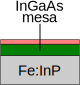
\includegraphics[width=\textwidth]{figures/Fabrication/fab1_1.pdf}
        \caption{\centering}
        \label{fig:fab11}
    \end{subfigure}
    \hfill
    \begin{subfigure}[b]{0.21\textwidth}
        \centering
        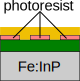
\includegraphics[width=\textwidth]{figures/Fabrication/fab1_2.pdf}
        \caption{\centering}
        \label{fig:fab12}
    \end{subfigure}
    \hfill
    \begin{subfigure}[b]{0.21\textwidth}
        \centering
        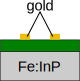
\includegraphics[width=\textwidth]{figures/Fabrication/fab1_3.pdf}
        \caption{\centering}
        \label{fig:fab13}
    \end{subfigure}
    \caption{Schematic diagram depicting the principle steps of structure lithography and metal deposition. (a) The wafer is covered in AZ 5214E photoresist. (b) UV exposure leaves behind a patterned photoresistive structure. A metal layer is deposited through metal evaporation on top of the photoresistive layer. (c) Lift-off is performed to get rid of the excess metal. Left behind is only the metal in contact with the semiconducting material.}
\end{figure}

A lithography mask is fabricated containing the desired antenna structures. A \num{7} $\times$ \num{8} \si{\milli\meter} sample of an InGaAs photoconductor, grown on a \num{500} \si{\micro\meter} InP:Fe substrate wafer is cleaved out from the wafer. In the following steps, structures as small as \num{5} \si{\micro\meter} are desired, so good contact and alignment are critical.

First, a fabrication step called zero-leveling is executed. The zero-leveling helps in achieving good contact when applying contact lithography. A thin layer of AZ 5214E image reversal photoresist is deposited onto the sample. By spin coating the sample at 8000 rpm, a uniform layer of photoresist is achieved. 
By soft baking the sample at \num{110} \si{\celsius} for one minute, it is prepared for ultraviolet (UV) exposure. 
The sample is exposed to UV light for \num{35} seconds, before being developed using AZ MIF 726, leaving a \num{5} $\times$ \num{6} \si{\milli\meter} area of photoresist.
A second lithographic step is carried out to define the antenna structures intended to be fabricated from chromium–gold (CrAu). The lithography mask is applied to the sample, which is then exposed to UV light for \num{3} seconds, followed by another soft baking step. A second UV exposure is carried out with five times the initial exposure duration. The sample is developed using AZ MIF 726, leaving behind the patterned antenna structures ready for CrAu deposition. 

The antenna structures are fabricated through metal deposition. Before depositing the metal for the PCAs, the samples are dipped into a 1:1 solution of H\textsubscript{2}O and HCl for \num{15} seconds to remove the oxide layer which forms at the surface. This step greatly improves the adhesion of the deposited metal. In the first metal deposition step, gold structures are deposited on top of a chromium adhesion layer. The antenna electrodes, contact pads and some part of the feeding strip are fabricated by depositing a \num{120} \si{\nano\meter} layer of gold (Au) on top of a \num{20} \si{\nano\meter} layer of Chrome (Cr) via thermal evaporation. Cr is deposited at a rate of $\sim 0.3$ \si{\angstrom}/\si{\s}, Au is deposited at a rate of $\sim 0.8$ \si{\angstrom}/\si{\s}. The Cr-layer improves the contact with the semiconducting material. After completing the metal deposition, the sample is placed in acetone and lift-off is performed. This way we get rid of the unwanted metal on our sample. 

An additional annealing step is performed after metal deposition to further improve the metal-semiconductor-contact. Such an annealing process reduces the interface impurities and creates good contact on the atomic scale between the metal and the semiconducting material \cite{tahamtanInvestigationEffectAnnealing2011}. Metal atoms diffuse into the InGaAs, making sure that we get an ohmic contact rather than a Schottky contact. Annealing is performed at a temperature of $\sim 422$ \si{\celsius} for \num{30} seconds under a nitrogen atmosphere at a pressure of \num{2} \si{\milli \bar}.  

\section{Mesa Lithography and Mesa Etching}

A layer of AZ 1518 HS photoresist is deposited onto the sample. Spin coating at 4000 rpm ensures a uniform photoresistive layer. Contact lithography is performed before hard baking the sample covered in photoresist at \num{110} \si{\celsius} for \num{15} minutes. By hard baking the sample, the resist is 
By hard baking the sample, the layer of photoresist is made more resistant to etching.   

The InGaAs photoconductive material is etched from the areas that were not protected by the photoresist layer using 
sulfuric acid (H\textsubscript{2}SO\textsubscript{4}), hydrogen peroxide (H\textsubscript{2}O\textsubscript{2}) and water (H\textsubscript{2}0) mixed in appropriate proportion. We use a ratio of \num{1} \si{\milli \liter} : \num{8} \si{\milli \liter} : \num{50} \si{\milli \liter} respectively. The semi-insulating InP:Fe substrate is left exposed in those areas. 

By mesa etching, the active InGaAs layer is removed from the entire sample except between the electrodes and under the antenna and pads. This process ensures a high resistance with a minimal dark current. A minimal dark current drastically improves the signal-to-noise ratio of the THz signal. 

\begin{figure}[!]
    \centering
    \begin{subfigure}[b]{0.21\textwidth}
        \centering
        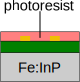
\includegraphics[width=\textwidth]{figures/Fabrication/fab2_1.pdf}
        \caption{\centering}
        \label{fig:fab21}
    \end{subfigure}
    \hfill
    \begin{subfigure}[b]{0.21\textwidth}
        \centering
        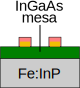
\includegraphics[width=\textwidth]{figures/Fabrication/fab2_2.pdf}
        \caption{\centering}
        \label{fig:fab22}
    \end{subfigure}
    \hfill
    \begin{subfigure}[b]{0.21\textwidth}
        \centering
        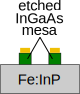
\includegraphics[width=\textwidth]{figures/Fabrication/fab2_3.pdf}
        \caption{\centering}
        \label{fig:fab23}
    \end{subfigure}
    \caption{Schematic diagram depicting the principle steps of structure lithography and metal deposition. (a) The wafer is covered in AZ 5214E photoresist. (b) UV exposure leaves behind a patterned photoresistive structure. A metal layer is deposited through metal evaporation on top of the photoresistive layer. (c) Lift-off is performed to get rid of the excess metal. Left behind is only the metal in contact with the semiconducting material.}
\end{figure}


\section{NiCr Structure Lithography and Deposition of NiCr}

This step is similar to the metal deposition of Au and Cr. The desired structures are imprinted onto the sample through photo-lithography. The imprinted structures are the missing parts of the feeding strips connecting antenna pads and electrodes. Good contact between the NiCr-strip and the AuCr-strip is vital. Otherwise, THz performance will decrease drastically. We spin coat the sample with nLof 2035 at \num{4000} rpm. The sample is soft baked, exposed to UV light and developed using AZ MIF 726. Left behind are the missing parts of the antenna feeding strips, ready for NiCr deposition.

A \num{80}/\num{20} NiCr alloy is deposited onto the sample using flash evaporation. Flash evaporation of \num{80}/\num{20} NiCr involves the rapid heating of the alloy in an evacuated environment (around $10^{-9}$ \si{\bar}). NiCr has a high melting point around \num{1450} \si{\celsius}. The alloy has to be heated rapidly to avoid clumps and bulk melting, assuring a thin, uniform NiCr layer on top of the sample. Constantly adjusting the feed rate of the alloy also helps in avoiding bulking. Ideally, the deposition rate should be kept as low as possible. In this work, the rate was kept at around \num{0.3} \si{\angstrom}/\si{\s}. As Nickel and chromium have slightly different melting temperatures it is also vital to make sure that the two metals are evaporated at equal rates.The 80/20 ratio is important to ensure that the NiCr alloy’s conductivity remains within the desired range. Upon reaching its evaporation temperature, the NiCr vaporizes, travels through the vacuum and accumulates on the sample surface.
\section{Anti-Reflection Coating Deposition}
\begin{wrapfigure}{r}{0.4\textwidth} % r = right side, 50% of text width
    \centering
    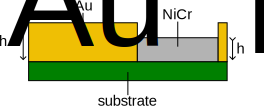
\includegraphics[width=0.39\textwidth]{figures/Fabrication/PCA_after_NiCr.pdf}
    \captionsetup{width=0.375\textwidth} % caption matches image width
    \caption{Schematic diagram of PCA cross section after NiCr deposition. The overlaps are idealized.}
    \label{fig:afterFab}
\end{wrapfigure}
An anti-reflection coating (ARC) is deposited above the active region. The ARC layer improves the absorption of the incoming infrared signal in the active region  \cite{chenAntireflectionImplementationsTerahertz2014} and protects the device from external damage. In the simplest implementation, an ARC consists of a single layer having the thickness of an odd multiple of the quarter-wavelength of the incident light: $d \sim k \frac{\lambda}{4}$. The refractive index of the coating material is chosen to be approximately the geometric mean of the indices of the two surrounding media. This choice ensures that the reflections occurring at the two interfaces are equal in magnitude and offset in phase. This leads to destructive interference and, consequently, reduced reflection (see Figure \ref{fig:fabarc}) \cite{paschottaAntireflectionCoatings2005}. 
The ARC is fabricated by growing a silicon nitride (Si\textsubscript{3}N\textsubscript{4}) layer on top of the sample via plasma-enhanced chemical vapor deposition (PECVD). Si\textsubscript{3}N\textsubscript{4} has a refractive index of $n_1 \approx 1.89$. We choose a thickness of $d = \frac{1}{4} \frac{\lambda}{n_1}$ for a wavelength of $\lambda = 1550$ \si{\nano \meter}, resulting  in a Si\textsubscript{3}N\textsubscript{4}-thickness of $d \approx 205$ \si{\nano \meter}. The Si\textsubscript{3}N\textsubscript{4}is deposited at a rate of approx. \num{13.5} \si{\nano \meter/\min}. After depositing the Si\textsubscript{3}N\textsubscript{4}, another layer of AZ 1518 HS photoresist is deposited onto the sample to form the required patterns of the Si\textsubscript{3}N\textsubscript{4} over the substrate. The photoresist covers the antenna’s electrode structure and feeding strip but leaves the pads uncovered. Otherwise, measurement of the received signal would not be possible. Photo-lithography is performed to acquire the needed structures. The Si\textsubscript{3}N\textsubscript{4} is etched out from the unprotected areas, exposing the contacting metal pads attached to the antenna. The etching is performed in a PECVD system in reactive ion etching (RIE) mode, using a carbon tetrafluoride (CF\textsubscript{4}) and oxygen (O\textsubscript{2}) plasma to chemically and physically remove the Si\textsubscript{3}N\textsubscript{4}. The unprotected Si\textsubscript{3}N\textsubscript{4} with a thickness of approx. \num{205}\,\si{\nano \meter} is etched in \num{55}\,\si{\s}. After etching of Si\textsubscript{3}N\textsubscript{4} the photoresist is removed by placing the sample in acetone.

\begin{figure}[!]
    \centering
    \begin{subfigure}[b]{0.21\textwidth}
        \centering
        \includegraphics[height=\textwidth]{figures/Fabrication/ARC_deposition_1.pdf}
        \caption{\centering}
        \label{fig:fabarc1}
    \end{subfigure}
    \hfill
    \begin{subfigure}[b]{0.21\textwidth}
        \centering
        \includegraphics[height=0.95\textwidth]{figures/Fabrication/ARC_deposition_2.pdf}
        \caption{\centering}
        \label{fig:fabarc2}
    \end{subfigure}
    \hfill
    \begin{subfigure}[b]{0.45\textwidth}
        \centering
        \includegraphics[width=\textwidth]{figures/Fabrication/ARC.pdf}
        \caption{\centering}
        \label{fig:fabarc}
    \end{subfigure}
    \caption{Schematic diagram depicting the deposition of an ARC and basic ARC working principle. (a) Silicon nitride deposition using a PECVD machine followed by deposition of a photoresistive layer. The photoresistive layer is transformed into structures covering the active region of the antennas using photo-lithography. (b) The silicon nitride is dry etched using carbon tetrafluoride to create the ARC. (c) Working principle of an ARC: incident light is reflected by the air-ARC interface and the ARC-substrate interface. The reflections destructively interfere. Not to scale.}
\end{figure}

\section{Dimensions of Processed Antennas}

\begin{itemize}
    \item umschreiben 
    \item bilder von antennen aufnehmen !!!
\end{itemize}

\begin{figure}[htbp]
    \begin{subtable}[c]{0.45\textwidth}
        \centering
        \begin{tabular}{l|l|l}
        \toprule
        Sample(s) & l\textsubscript{NiCr} [$\mu m$] & l\textsubscript{CrAu} [$\mu m$] \\
        \midrule
        H5, H9, H10 & 0 & 751.5 \\
        H4 & 5 & 746.5 \\
        H1, H2 & 10 & 741.5 \\
        H6 & 15 & 736.5 \\
        H3, H8 & 70 & 701.5 \\
        H7 & 240 & 511.5 \\
        \bottomrule
        \end{tabular}
        \caption{\centering H-Dipole Dimensions}
        \label{tab:table}
    \end{subtable}
    \hspace{0.1em}
    \begin{subtable}[c]{0.45\textwidth}
        \centering
        \begin{tabular}{l|l|l}
        \toprule
        Sample(s) & l\textsubscript{NiCr} [$\mu m$] & l\textsubscript{CrAu} [$\mu m$] \\
        \midrule
        D1, D6 & 0 & 751.5 \\
        D3, D8 & 70 & 701.5 \\
        D4, D9 & 240 & 511.5 \\
        D5, D10 & 500 & 251.5 \\
        D2, D7 & 721.5 & 30 \\
        \bottomrule
        \end{tabular}
        \caption{\centering I-shaped Dipole Dimensions}
        \label{tab:table}
    \end{subtable}
    \caption{}
    \label{fig:sim_dimensions}
\end{figure}

We present the dimensions of the processed H-Dipole and I-shaped Dipole antennas based on the performed simulations. In total, 11 H-Dipole antennas and 13 I-shaped Dipole antennas are processed, partly differing in geometry. Table \ref{} displays the fabricated antennas and their corresponding dimensions important for this work. All of the processed antennas exhibit a strip width of \num{5}\,\si{\micro \meter}. All read-out pads are fabricated as squares, measuring \num{196}\,\si{\micro \meter} $\times$ \num{196}\,\si{\micro \meter}. The total strip length of H-Dipoles and I-shaped Dipoles measures \num{1900}\,\si{\micro \meter}, resulting in an effective strip length of \num{1508}\,\si{\micro \meter} in between the pads. One exception to this rule is an I-shaped Dipole antenna fabricated without adding any NiCr but with increased effective strip length measuring \num{4508}\,\si{\micro \meter}.


\section{DC Characterization}
By DC characterizing the fabricated antennas we aim to ensure ohmic behavior. The IV-characteristics of the antennas are measured by sweeping through the supply voltage from \num{-1000} \si{\milli \volt} to \num{1000} \si{\milli \volt} with a step size of \num{50} \si{\milli \volt}. Figure \ref{fig:main_IV_dipoles} shows the measured dark current $I_{DC}$ over the applied voltage $V$. Each plot displays two antennas with similar properties, meaning identical fabrication. All antennas display ohmic behavior as their IV-characteristics are strictly linear, thus $I_{DC} \sim V$ and $R = \frac{\Delta V}{\Delta I_{DC}}$. We conclude that concerning the metal-semiconductor contact, the antennas behave as expected.  

The measured resistance is generally higher than assumed in simulations. The sheet resistance can be calculated from the measurements as follows

\begin{equation}
    R_{sq} = R_{NiCr}\cdot\frac{w_{strip}}{l_{NiCr}},
\end{equation}

where $w_{strip}$ is the width of the feeding strip, $l_{NiCr}$ is the length of the NiCr portion of the strip and $R_{NiCr}$ is the measured resistance. By calculating the sheet resistance for every measurement of H-Dipole antennas with NiCr induced feeds and taking the mean, we arrive at a sheet resistance of approx. $R_{sq} = 215$ \si{\ohm/sq}. Compared to the assumptions in our simulations, the sheet resistance is approx. ten times higher than expected. The assumed sheet resistance in simulations stemmed from previous flash evaporation processes and measurements. The flash evaporation for this thesis was done at slightly lower temperatures. This results in different conductivity properties of the \num{80}/\num{20} NiCr alloy and could be a reason for the higher sheet resistance.

\textbf{TODO: REWORK !!!!}


In simulations we saw that above a few hundred ohms we should expect the low frequency resonances to reduce and ultimately disappear. With the now fabricated antennas, we expect to only observe low frequency resonances in the reference H-Dipole that does not contain NiCr. Even the antenna with the shortest NiCr-strip $L_{NiCr} = 70$ \si{\micro \meter} should already completely suppress the undesired low frequency effects caused by the pads. What happens with the resistances around \num{20} \si{\kilo \ohm} has to be evaluated in measurements. The NiCr strips act as an additional parallel resistance to the resistance of the photoconductor $R_P$ (see figure \ref{PCA_eq}). Usually, $R_P$ is in the mega ohm region and can be ignored as it is parallel to the radiation impedance $Z_A$ of the antenna. In eq. \ref{transferfunction} we assumed $R_P \gg R_A$, so $R_P$ could be neglected. With small values for $R_{NiCr}$ however, the parallel circuit of $R_P$ and $R_{NiCr}$ is

\begin{equation}
    R_{res} = R_P || R_{NiCr} = \frac{R_P\cdot R_{NiCr}}{R_P + R_{NiCr}} \approx R_{NiCr}.
\end{equation}

We cannot assume to neglect the resistance parallel to $R_A$ anymore. Inserting this result into eq. \ref{transferfunction} we get 

\begin{equation}
    H = \frac{Z_{out}}{Z_{in}} = \frac{\frac{1}{i\omega C_P}}{R_A || R_{NiCr} + \frac{1}{i\omega C_P}} = \frac{1}{1 + i\omega C_P \frac{R_A \cdot R_{NiCr}}{R_A + R_{NiCr}}} = \frac{1}{1 + i 2\pi \nu_{THz} \tau_{RC}}.   
\end{equation}

We see that the transfer function of the PCA is only influenced when $R_{NiCr}$ is sufficiently small. 

\begin{figure}[ht]
    \centering
    \includegraphics[width=0.7\textwidth]{figures/eq_circuit_PCA_wNiCr.pdf}
    \caption{}
    \label{eq_circuit_NiCR}
\end{figure}

\begin{figure}[ht]
    \centering

    \begin{subfigure}[b]{0.49\textwidth}
        \centering
        \includegraphics[width=\textwidth]{figures/IV/IV_H1_H6.pdf}
        \caption{IV characteristics of H-Dipole antennas with a NiCr-strip of length $l_{NiCr} = 500$ \si{\micro \meter}.}
        \label{fig:sub1}
    \end{subfigure}
    \hfill
    \begin{subfigure}[b]{0.49\textwidth}
        \centering
        \includegraphics[width=\textwidth]{figures/IV/IV_H2_H7.pdf}
        \caption{IV characteristics of H-Dipole antennas with a NiCr-strip of length $l_{NiCr} = 240$ \si{\micro \meter}.}
        \label{fig:sub2}
    \end{subfigure}
    
    \vspace{1em} % space between rows

    \begin{subfigure}[b]{0.49\textwidth}
        \centering
        \includegraphics[width=\textwidth]{figures/IV/IV_H3_H8.pdf}
        \caption{IV characteristics of H-Dipole antennas with a NiCr-strip of length $l_{NiCr} = 70$ \si{\micro \meter}.}
        \label{fig:sub3}
    \end{subfigure}
    \hfill
    \begin{subfigure}[b]{0.49\textwidth}
        \centering
        \includegraphics[width=\textwidth]{figures/IV/IV_H4_H9.pdf}
        \caption{IV characteristics of H-Dipole antennas with a NiCr-strip of length $l_{NiCr} = 751$ \si{\micro \meter}.}
        \label{fig:sub4}
    \end{subfigure}
    
    \vspace{1em} % space between rows

    \begin{subfigure}[b]{0.49\textwidth}
        \centering
        \includegraphics[width=\textwidth]{figures/IV/IV_H5_H10.pdf}
        \caption{IV characteristics of H-Dipole antennas with a NiCr-strip of length without added NiCr.}
        \label{fig:sub5}
    \end{subfigure}

    \caption{Measured IV characteristics of the fabricated H-Dipole antennas.}
    \label{fig:main_IV_dipoles}
\end{figure}


\chapter{Results and Discussion}

\textbf{TODO: rework Intro}

The setup used for Measuring THz radiation using a pulsed system is presented in the following. Measurements of the proposed antennas are evaluated by analyzing anc comparing their transient behavior. 

\section{THz TDS Measurement Setup}
\begin{figure}[ht]
    \includegraphics[width=0.9\linewidth]{figures/TDS_schematic.pdf}
    \centering
    \caption{Schematic diagram of the setup used for THz-TDS.}
    \label{fig_TDS}
\end{figure}

Generation and detection of THz radiation in a pulsed system were described in detail in Section \ref{sec_gen_det}. Only a brief overview will be given here. The TSD setup (see Figure \ref{fig_TDS}) used for characterization of the fabricated H-Dipole antennas utilizes a modified MenloSystems C-Fiber \cite{FemtosecondErbiumLaser} laser system with a pulse duration of \num{90} \si{\femto \s}, a repetition rate of \num{100} \si{\mega \hertz} and an optical wavelength of \num{1560} \si{\nano \meter}. The laser signal is coupled out using glass fibers. In order to achieve coherent signal detection, the THz-TDS setup utilizes a closed-loop system. Both the pump beam and the probe beam necessary for THz generation and detection with PCAs are generated using the same laser beam. The fibers drive both the detector and the emitter with \num{25} \si{\milli \watt} of power each. The THz signal is generated with the help of the pump beam and ultimately detected by sampling the temporal overlap of the probe beam and the THz field. This closed-loop approach ensures that the THz-TDS system provides high SNR and DNR. A beam splitter is utilized to split the initial laser pulse into the two needed signals. 

On the transmission side of the setup, one of the two laser signals passes through a delay stage before being fed into the transmitter (Tx) developed in \cite{nandiErAsInAlGaAsPhotoconductors2021}. The transmitter primarily consists of a PCA mounted on a hyper-hemispherical silicon lens with a radius of \num{6.1} \si{\milli \meter}. The device is fully packaged, featuring an APC-fiber for the laser signal and a SMA connector for applying the bias voltage. The package has a cylindrical shape with a length of \num{5} \si{\centi \meter} and an outer diameter of \num{6} \si{\centi \meter}. Additionally, the packaging includes a fiber collimator and a focusing lens to ensure efficient coupling of the laser signal into the device. The PCA is DC-biased until a current of approximately $180$ \si{\micro \ampere} is reached, enabling the acceleration of free charge carriers generated by the laser signal. This typically corresponds to a bias voltage of around \num{180} \si{\volt}. The fully packaged transmitter is mounted on a one-dimensional stage to horizontally align the THz field. When illuminated by the laser signal, the PCA emits THz radiation. The THz field travels through free space and is focused onto the receiving port by two lenses.  

As demonstrated in Section \ref{sec_gen_det}, the signal at the receiver in this setup can be approximated as the convolution of the delta-function and the incident THz transient. Hence, a mechanical delay stage is needed before the laser signal reaches the transmitter to scan through the complete THz pulse. By varying the relative delay between the THz signal and the optical probing pulse, the complete THz pulse received by the antenna can be extracted. 

The second laser signal is directly coupled to the receiving port (Rx) of the setup. The receiver consists of an antenna that is being used to work as a recipient for THz radiation.  In this thesis, the receiving port of the setup is an antenna of the fabricated probe, which serves as the device under test (DUT). The DUT is mounted on a hyper-hemispherical silicon lens with a radius of \num{6.1} \si{\milli \meter}, using vacuum grease for attachment. A fiber collimator and a focusing lens are employed to direct the laser pulse onto the active region of the DUT. Two three-dimensional stages are used: one for aligning the laser signal with the DUT, and another for aligning the DUT with the incident THz transient.

For a PCA to work as a receiver, the device is illuminated by the femtosecond laser pulse, the probing pulse. By illuminating the device, free electron-hole pairs are generated. The incoming THz radiation, which is to be measured by the receiving port, biases the device. The illumination and biasing of the device results in a DC photocurrent. This current is proportional to the convolution of the incoming THz transient and the optical probing signal. The DC current can be read out using probing needles at the antenna pads and post detection electronics. As the measured photocurrent is generally very small (around $10^{-9} ... 10^{-6}$ \si{\ampere}), the signal is transformed to a voltage and amplified by a trans-impedance amplifier (TIA) from TEM-Messtechnik (PDA-S) \cite{PDASPhotodiodenVerstaerker}. With the TIA, gains of up to $\sim 10^7 $ \si{\volt}/\si{\ampere} can be achieved. The THz signal needs to be extracted from background noise. A Lock-In Amplifier (LIA) is used for signal extraction. The input signal is multiplied with a reference signal (demodulation), which is usually a sine-wave, and then filters the result using a low-pass filter. This isolates the desired signal at a specific frequency from noise and other frequency components. The frequency at which the demodulation takes place is the same frequency used for modulating the THz transmitter. A LIA from Zurich Instruments (MFLI-MD) \cite{MFLI500KHz2019} is employed for demodulation of the incoming signal. A graphical user interface provided by MenloSystems is used for data acquisition and storage. For all measurements, a scanning window of \num{100} \si{\pico \s} is employed. The data is recorded with an integration time of \num{1000} \si{\s} to achieve the highest possible SNR. The time-domain data is saved for further data analysis.


\chapter{Summary and Outlook}

\printbibliography

\end{document}
